A continuación procedemos a cuantificar la importancia de la limpieza de la superficie de las fibras. El motivo de ello es que, para el proyecto Tritium, que utiliza fibras sin clad, el estado de la superficie es muy impotante ya que esta \textit{interface} formada entre el clad y el agua tritiada será la que marcará la mayor o menor tasa de conservación de los fotones. Lo mismo ocurrirá para fibras con single clad o multi clad, pero de forma menos importante.

La forma con la que pretendemos cuantificar la importancia del tratamiento de las superficies de las fibras será repetir la sección \ref{sec:sigmaint} pero, en cada fibra sometida a estudio, se incluirá una exhaustiva tarea de limpieza con ayuda de alcohol 2-isopropanol. Unicamente se realizará para un tipo de fibra, single clad, debido al tiempo que se necesita para llevar a cabo esta tarea. Se realizará sobre el tipo single clad ya que, en esta, se encontró una confrotación de los resultados obtenidos para la señal entre dos estudios anteriores.

Por tanto, preparamos 10 muestras diferentes de fibras single clad de $20~\cm$ y, con ayuda de alcohol y unos pañuelos especialmente preparados para su utilización en salas blancas, realizamos una exhaustiva limpieza sobre la superficie de cada fibra.

De forma análoga a la sección \ref{sec:sigmaint} mostramos a continuación los resultados del experimento:

\begin{figure}[hbtp]
\centering
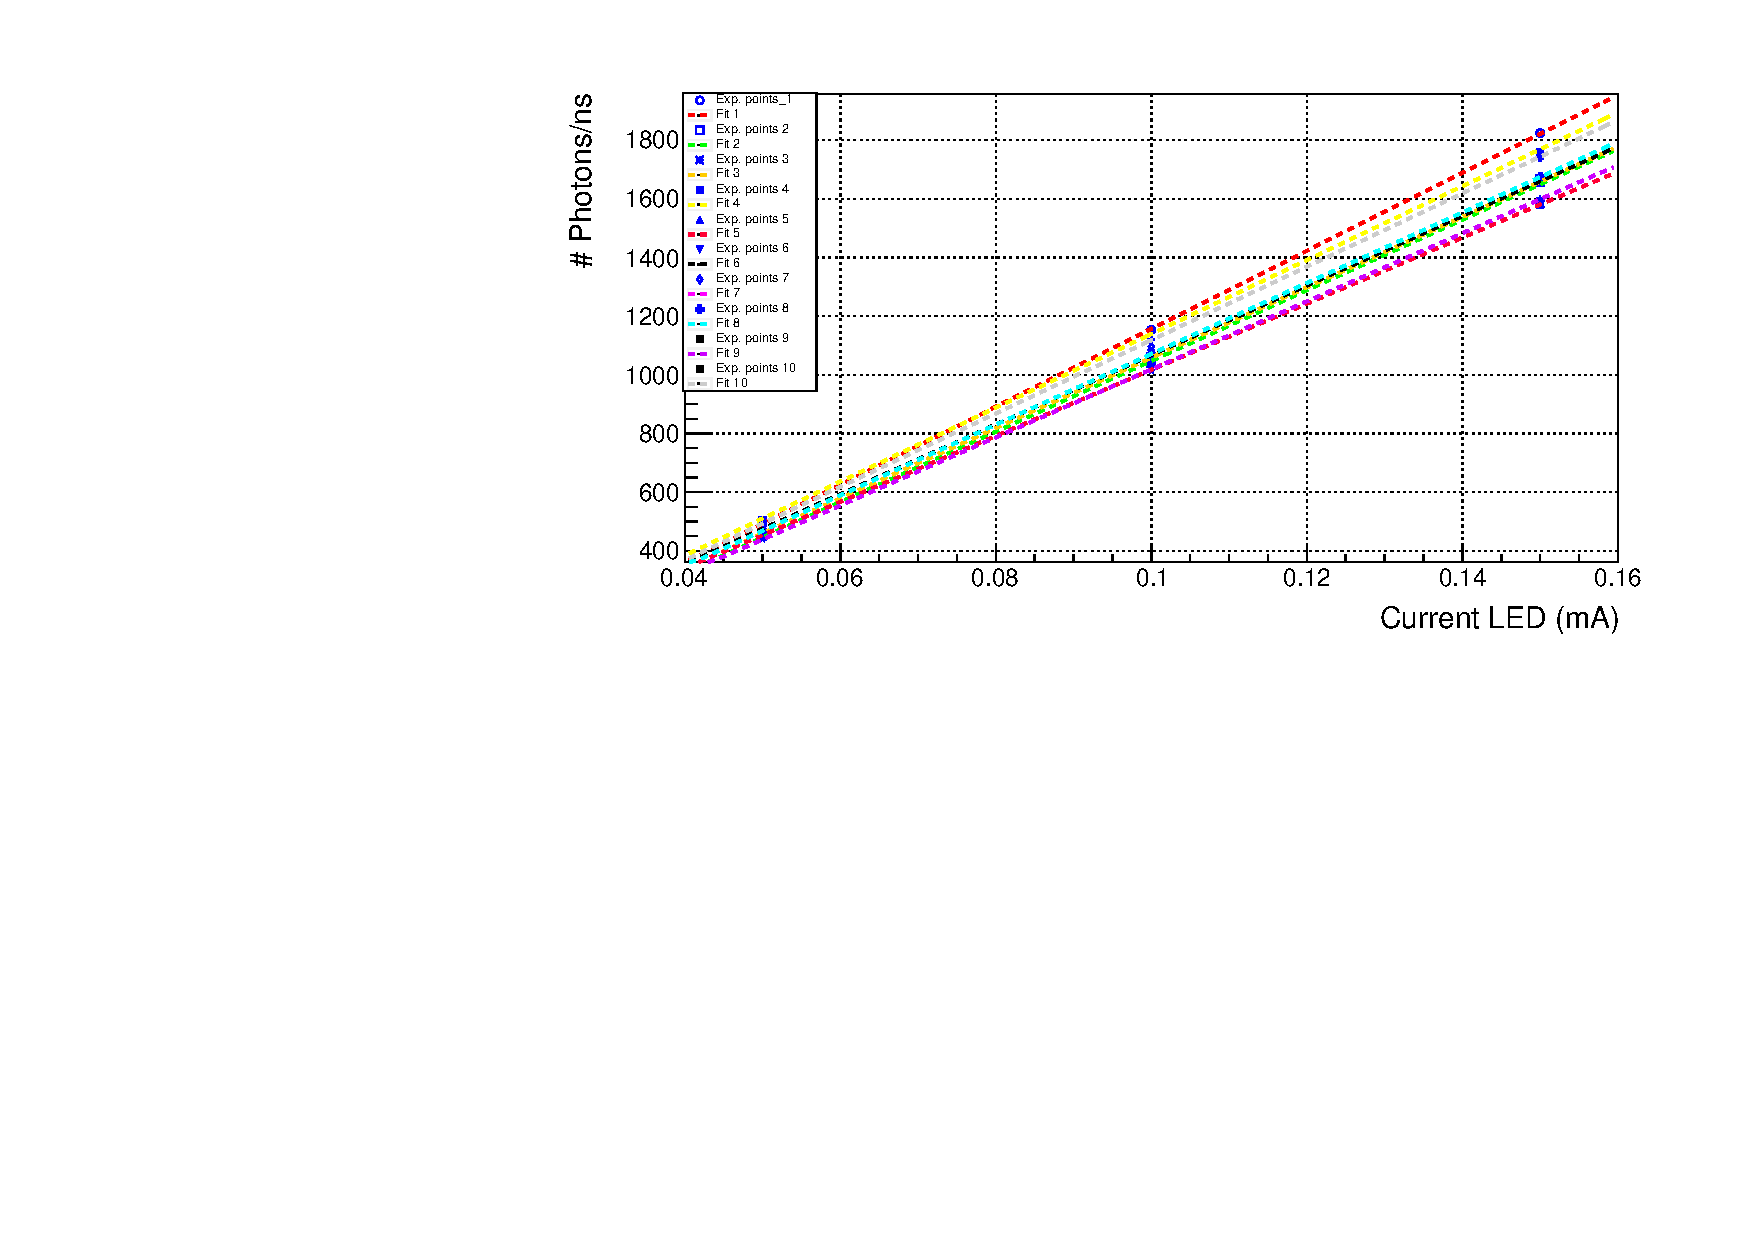
\includegraphics[scale=0.7]{Figuras/SamplesSingleCladMarcos.pdf}
\caption{Intensidad obtenida en 10 muestras diferentes de fibras single clad de $200~\mm$ frente a la alimentaicón de la LED con la implementación del tratamiento de superficie\label{medidassinglecladlimpieza}}
\end{figure}

De nuevo observamos una perfecta linealidad de la señal en cada una de las fibras frente a la alimentación de la LED. Con ayuda de las expresiones \ref{ecuacionmedia} y \ref{ecuaciondesviacionestandar} obtenemos su promedio y desviación estandar. Los resultados se muestran en la tabla \ref{singlecladlimpieza}, donde se incluyen los resultados anteriores obtenidos sin la implementación de este tratamiento de las superficies:

\begin{table}[H]
\begin{center}
\begin{tabular}{l | c | c | c | c }
Intensidad LED $(\milli\ampere)$ &  Sin tratamiento $(N.\gamma~/\nano\second)$ & Con tratamiento $(N.\gamma~/\nano\second)$ \\
\hline \hline
$0.05$ & $383.81 \pm 33.23$ & $470.60 \pm 6.57$\\ 
$0.1$ & $922.68 \pm 73.97$ & $1082.28 \pm 14.27$\\
$0.15$ & $1485.10 \pm 119.90$ & $1681.65 \pm 24.82$\\
$0.2$ & $2053.78 \pm 166.391$ & $ --- $\\

\end{tabular}
\caption{Señal y desviación estandar para fibras single clad con y sin tratamiento de la superficie para cada alimetnación de la LED\label{singlecladlimpieza}}
\end{center}
\end{table}

Podemos notar la sutileza que ahora no se ha llegado a medir el caso de $0.2~\milli\ampere$. El motivo de ello fueron una serie de complicaciones técnicas. Sin embargo, debido a la alta linealidad de la respuesta del sistema, podemos considerar que estas complicaciones no afectarán de forma significativa al resultado del experimento. Seguidamente resumimos esta tabla en un gráfico donde se muestran ambas señales superpuestas: 

\begin{figure}[hbtp]
\centering
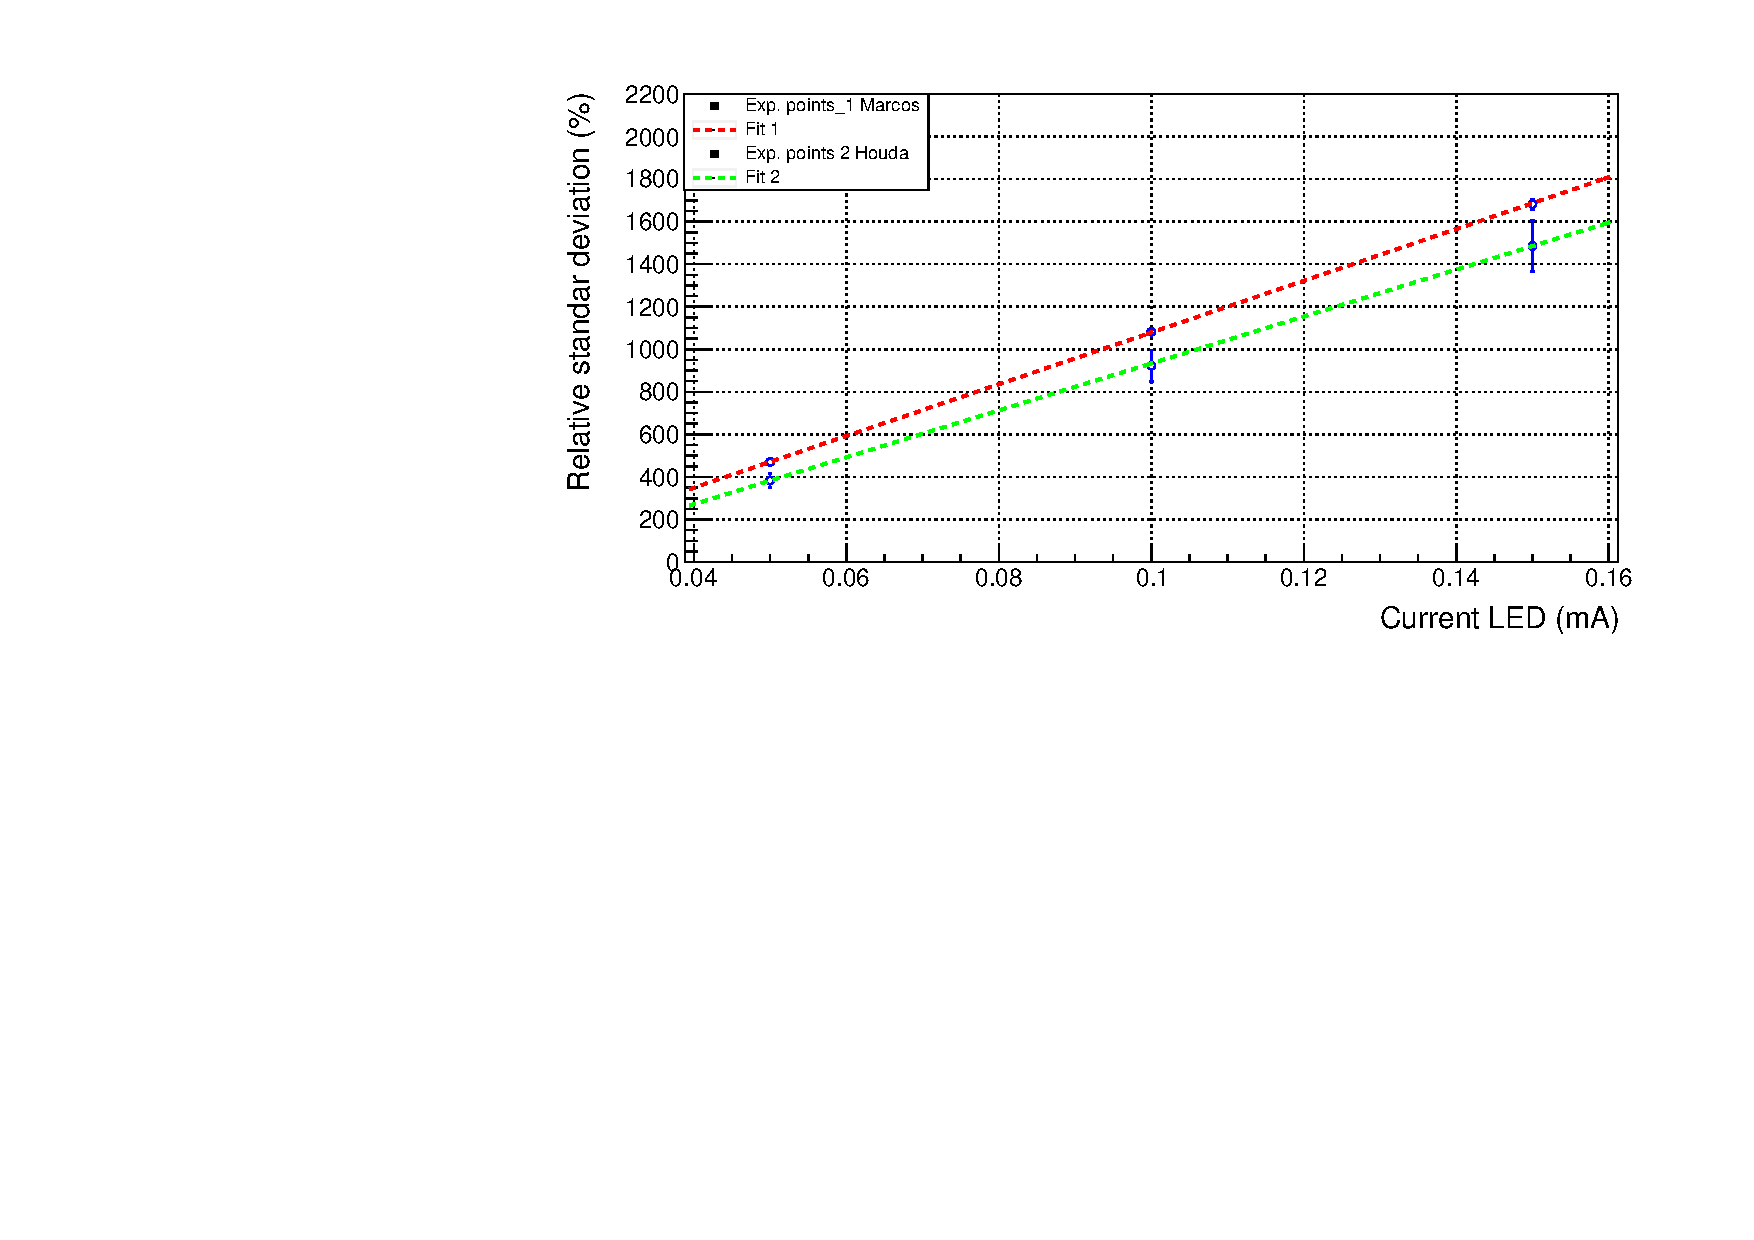
\includegraphics[scale=0.7]{Figuras/comparacion.pdf}
\caption{Intensidad promediada de 10 muestras diferentes de fibras single clad de $200~\mm$ frente a la alimentaicón de la LED con y sin la implementación del tratamiento de superficie\label{promediosinglecladlimpieza}}
\end{figure}

Podemos observar, en primer lugar, un lijero aumento de la señal obtenida con dichas fibras. La razon de ello es, como ya se ha explicado, una mejora de la eficiencia de recolección. En segundo lugar, podemos apreciar una considerable reducción  de las incertidumbres asociadas a cada uno de los promedios, algo realmente importante desde el punto de vista del proyecto Tritium ya que este busca trabajar con un número considerable de fibras. 

En último lugar incluimos la tabla \ref{comparacionincertidumbres} donde se presentan las distintas desviaciones estandar relativas obtenidas en cada caso:

\begin{table}[H]
\begin{center}
\begin{tabular}{l | c | c | c | c }
Person & $\sigma_{total} (\%) $ & $\sigma_{pos} (\%)$\\
\hline \hline
Con tratamiento & 1.4  & 2.17\\ 
Sin tratamiento & 8.2 & 2.17\\
\end{tabular}
\caption{Desviaciones estandar relativas obtenidas para cada caso\label{comparacionincertidumbres}}
\end{center}
\end{table}

En primer lugar podemos ver que se ha verificado la confrotación de resultados en la señal debida al caso single clad. Además, en segundo lugar, podemos observar que, con la implementación de un exhaustivo método de tratamiento de la superficie previo al momento de la realización de la medida se ha conseguido disminuir la incertidumbre hasta en un $82.93\%$, factor muy importante y de gran implicación en el proyecto Tritium. De hecho, su reducción fue tal que imposibilito la obtención de la desviación estandar debida al proceso de preparación de las fibras, el cual lo obtenemos con ayuda de la ecuación \ref{incertidumbreint}, por el simple hecho que obtenemos un valor negativo en el interior de la raiz. 

Debido a ello necesitamos recalcular la desviación estandar asociada a la posición de la fibra en el SetUp con la implementación de este proceso de tratamiento de la superficie. De manera totalmente análoga a la sección \ref{sec:sigmapos} presentamos los resultados en el siguiente histograma:

\begin{figure}[hbtp]
\centering
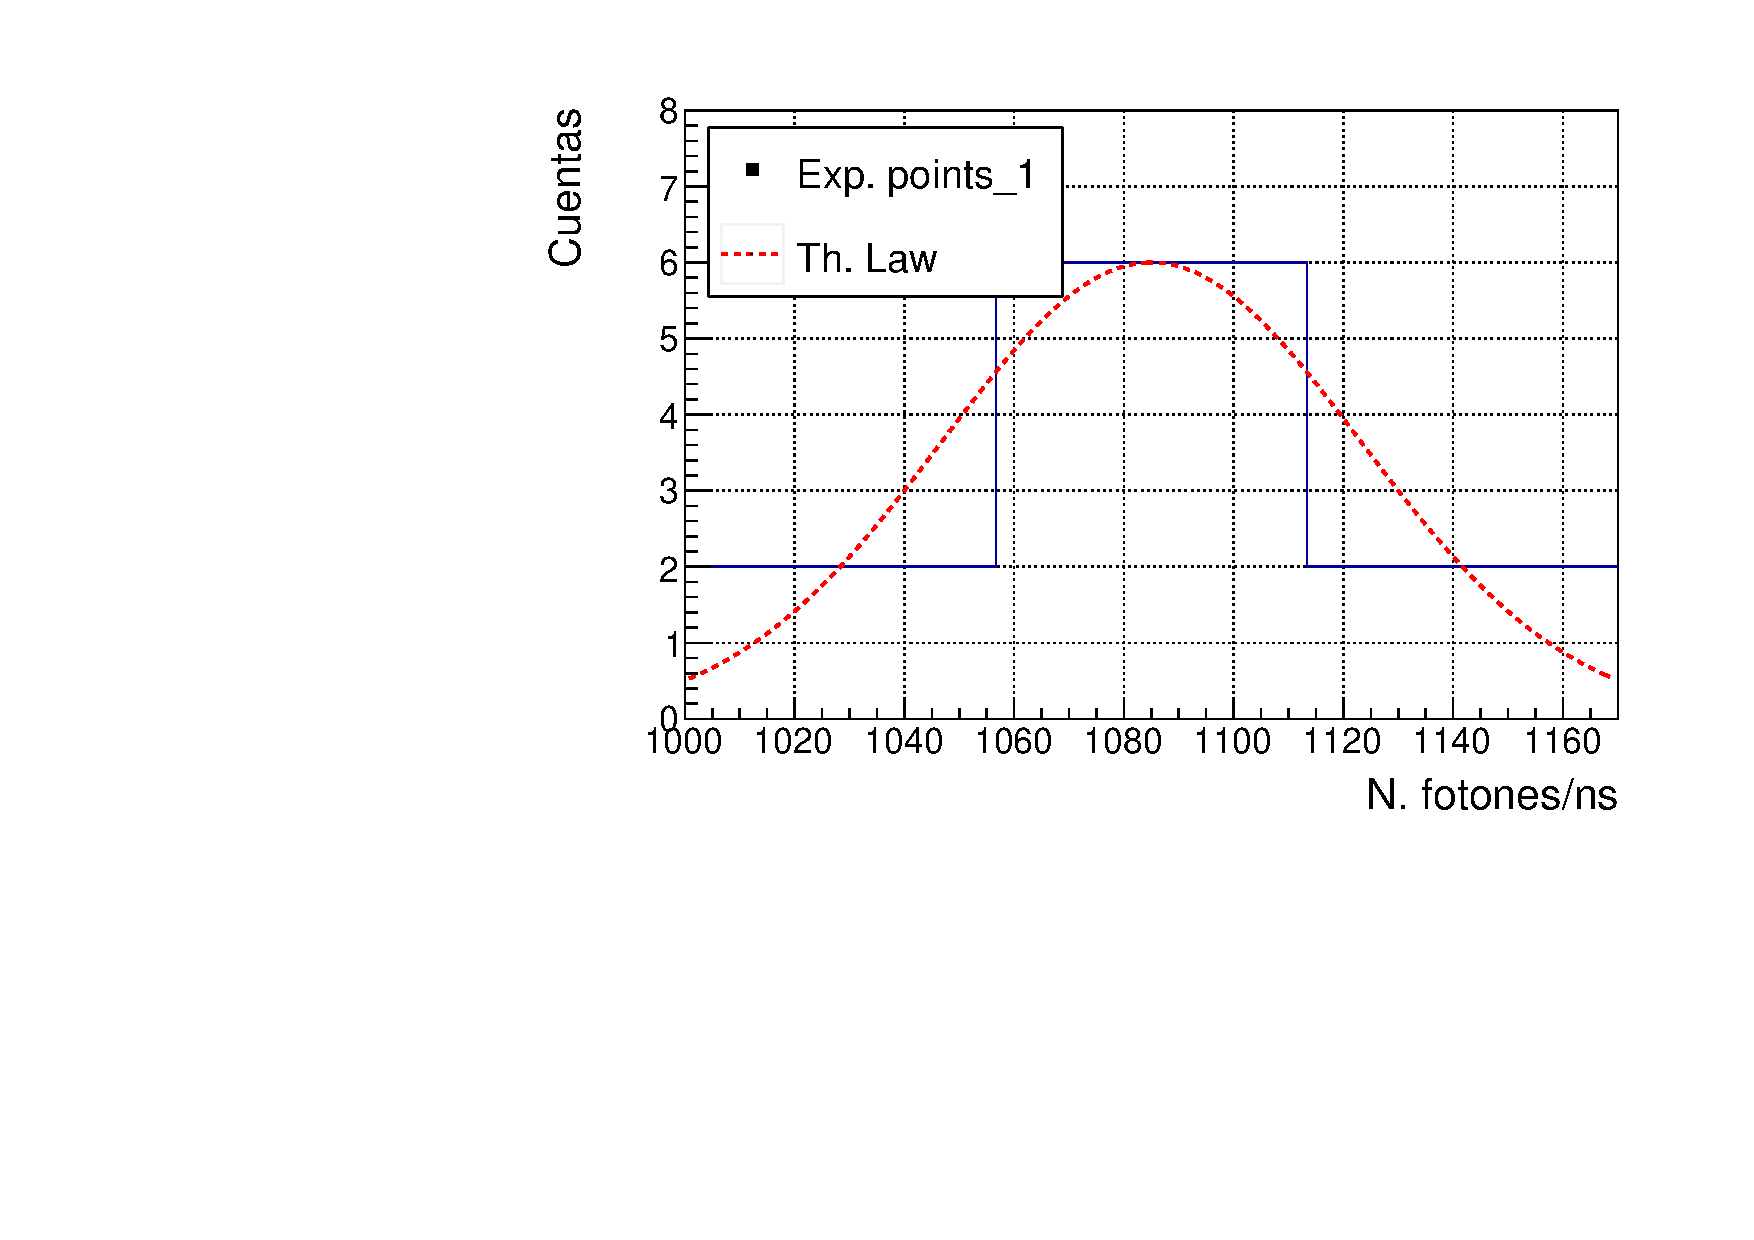
\includegraphics[scale=0.7]{Figuras/singlecladsigmaposgausclean.pdf}
\caption{Intensidad promediada de 10 muestras diferentes de fibras single clad de $200~\mm$ frente a la alimentaicón de la LED con y sin la implementación del tratamiento de superficie\label{promediosinglecladlimpieza}}
\end{figure}

Donde, con ayuda de las ecuaciones \ref{ecuacionmedia} y \ref{ecuaciondesviacionestandar}, obtenemos un resultado de $S=1071.70~\pm~9.07~N. \gamma/\nano\second$, resultado que, de nuevo, confirma la confrotación entre resultados que obtuvimos en el pasado.

 Podemos observar que se ha obtenido un valor para la desviación estandar relativa de $0.85\%$, valor considerablemente menor que el caso anterior. Por tanto vemos que, con la implementación del tratamiento de la superficie conseguimos una reducción de la incertidumbre asociada a la posición de hasta un $61\%$, valor que nos confirma nuevamente que el método de tratamiento de la superficie de la fibra funciona.
 
Finalmente, con ayuda de este valor y de la ecuación \ref{incertidumbreint}, obtenemos la desviación estandar debida únicamente al proceso de preparación de las fibras. Este resultado, junto con el caso anterior sin tratamiento, se muestra en la tabla \ref{resultadofinalclean}:

\begin{table}[H]
\begin{center}
\begin{tabular}{l | c | c | c | c }
Person & $\sigma_{total} (\%) $ & $\sigma_{pos} (\%)$ & $\sigma_{int} (\%)$\\
\hline \hline
Con tratamiento & 1.4  & 0.85 & 1.11\\ 
Sin tratamiento & 8.2 & 2.17 & 7.91\\
\end{tabular}
\caption{Desviaciones estandar relativas obtenidas para cada caso\label{resultadofinalclean}}
\end{center}
\end{table}

Vemos por tanto que ha quedado demostrada la notable disminución de la desviación standar de la señal asociada a la fibras al incluir en su protocolo de preparación un tratamiento para las superficies. Debido a ello, en la construcción del prototipo Tritium 1, se desarrolló e incluyo un método de tratamiento de las superficies de cada una de las fibras que se utilizó. Este método se explica en la sección \ref{sec:limpiezaICMOL}.